% ====================================================================
%                                                                 
%
%       §01
%
%
% %%ts latex start%%[2019-03-07 Thu 14:45]%%ts latex end%%
% ====================================================================


% --------------------------------------------------------------------
% §1.1 section <<Begriff der Relation>>
% --------------------------------------------------------------------
\section{Begriff der Relation}

Im letzten Kapitel haben wir Ausdrücke der Form $f(x)=x^3$ in \textit{Abbildungen} $f:A\to B$ verallgemeinert, die eine Beziehung zwischen den Elementen einer Menge $A$ und einer Menge $B$ herstellen. Heute möchten wir Ausdrücke wie $2\leq 3$ oder $\sqrt{2}\neq \sqrt{3}$, die Beziehungen zwischen je zwei Elementen der selben Menge angeben, als \textit{Relationen} realisieren. Relevant sind vor allem \textit{Ordnungsrelationen} und \textit{Äquivalenzrelationen}.

% Definition Relation
Abstrakt kodieren wir für den Relationenbegriff die Elemente, die in Beziehung
stehen sollen, in einem Paar, also einem Element des kartesischen
Produkts.
\begin{de}
	Sei $X$ eine Menge. Eine \textbf{Relation} $\sim$ auf $X$ ist verkörpert durch eine Teilmenge $R\subseteq X\times X$ mit
\begin{align*}
 x\sim y\quad :&\Leftrightarrow\quad (x,y)\in R && x,y\in X
\end{align*}
\end{de}

%\begin{bsp}\label{bsp:gatsby}
%	Auf der Menge $X=\{\text{Nick Carraway, Jay Gatsby, Daisy Buchanan, Thomas Buchanan}\}$ betrachten wir die Relation \glqq\,$\_$ liebt $\_$\grqq\,. Wir haben $N$ liebt $J$, $D$ liebt $J$, $J$ liebt $D$ und $T$ liebt $D$.
%		\[ \begin{tikzcd}
%			N \ar[r] & J \ar[d,leftrightarrow]\\ T \ar[r] & D
%		\end{tikzcd} \]
%	Die kodierende Menge $R\subset X\times X$ ist also
%		\[ R = \left\{(N,J),(J,D),(D,J),(T,D)\right\} \,. \]
%\end{bsp}

\begin{bsp}\label{bsp:starwars}
	Auf der Menge $X=\{$Luke Skywalker, Anakin Skywalker, Yoda, Obi-Wan Kenobi, Qui-Gon Jinn, Dooku, Palpatine, Darth Maul, Darth Plagueis$\}$ betrachten wir die Relation
		\[ x \sim y :\Longleftrightarrow \text{ $x$ war Padawan von $y$. } \]
	Wir haben
		\[\begin{tikzcd}
			&		& \text{Darth Plagueis} & \\
			& \text{Yoda} & \text{Palpatine} \ar[u] & \\
			& 		& \text{Dooku}\ar[u]\ar[ul] & \text{Darth Maul}\ar[ul] \\
			&		& \text{Qui-Gon Jinn} \ar[u] &\\
			&		& \text{Obi-Wan Kenobi} \ar[u] & \\
			& \text{Luke Skywalker}\ar[uuuu]\ar[ur]	& &\text{Anakin Skywalker}\ar[ul]\ar[uuuul]
		\end{tikzcd}\]
	Ein Pfeil von $a$ nach $b$ soll dabei dafür stehen, dass $a$ mit $b$ in Beziehung $a\sim b$ steht, also $a$ ein Padawan von $b$ war. Eine solche Darstellung nennt man einen \textbf{Graphen} der Relation.
	
	Die kodierende Menge $R\subset X\times X$ ist also $R = \big\{$(Luke,Yoda), (Luke,Obi-Wan), (Anakin,Obi-Wan), (Anakin, Palpatine), (Obi-Wan,Qui-Gon), (Qui-Gon, Dooku), (Dooku, Yoda), (Dooku, Palpatine) (Darth Maul, Palpatine), (Palpatine, Darth Plagueis)$\big\}$.
\end{bsp}

\begin{bsp}\label{bsp:leq}
	Auf $\Zz$ definieren die Relation \glqq$\leq$\grqq\, durch
\begin{align*}
 n\leq m \quad &:\Leftrightarrow\quad \exists k\in\mathbb{N}_0: m=n+k  && n,m\in \Zz
\end{align*}
	Durch welche Menge $R\subset\Zz\times\Zz$ wird \glqq$\leq$\grqq\, repräsentiert? Für $n,m\in \Zz$ gilt: 
		\[ (n,m)\in R\quad \overset{!}{\Leftrightarrow}\quad n\leq m \quad\Leftrightarrow\quad \exists k\in\mathbb{N}_0: m=n+k \,. \]
	Eine mögliche Formulierung wäre also \( R = \left\{(n,m)\in\Zz\times\Zz\mid\exists k\in\mathbb{N}_0: m=n+k\right\} \). Letztlich haben wir hier einfach nur die Definition der Relation abgeschrieben und nicht wirklich etwas gelernt; wenn man tatsächlich mit Relationen arbeitet, ist es ganz allgemein meist ergiebiger, die Menge $R$ als technische Umsetzung zu vergessen und sich mit der direkten Definition der Relation auseinanderzusetzen. Wie das gemeint ist, sehen wir gleich bei den Eigenschaften von Relationen.
\end{bsp}

\begin{de}\label{bsp:trivialrelationen}
	Vorher noch drei Extrembeispiele: Sei $X$ eine beliebige Menge.
\begin{itemize}
 \item Die \textbf{Allrelation} auf $X$ ist verkörpert durch die Menge $X\times X$, setzt also alle Elemente miteinander in Beziehung:
		\[ \begin{tikzcd}[column sep = huge]
			x \ar[loop] \ar[r,<->] \ar[rr, out=320, in=220, <->] &
			y \ar[loop] \ar[r,<->]  &
			z \ar[loop] 
		\end{tikzcd} \]
	Die Doppelpfeile stehen dabei für eine Beziehung in beide Richtungen, etwa gilt $x\sim y$ sowie $y\sim x$.
\item Die \textbf{Nullrelation} ist verkörpert durch die leere Menge $\emptyset$, setzt also keine Elemente in Beziehung:
		\[ \begin{tikzcd}[column sep = huge]
			 x &y &z &  
		\end{tikzcd} \]
\item Die \textbf{Gleichheitsrelation} ist definiert durch $x\sim y:\Leftrightarrow x=y$, also
		 \[ \begin{tikzcd}[column sep = huge]
		 	x \ar[loop] &
		 	y \ar[loop] &
		 	z \ar[loop] 
		 \end{tikzcd} \]
	Sie ist verkörpert durch die so genannte \emph{Diagonale}
		\[ D_X :=\left\{ (x,x)\in X\times X\mid x\in X \right\} \,. \]
	(In der Darstellung des kartesischen Produkts als Ebene mit Koordinatenachsen ist das gerade die Winkelhalbierende, daher der Name.)
\end{itemize}
\end{de}

\begin{de}
	Sei $X$ eine Menge und $\sim$ eine Relation auf $X$. Dann heißt die Relation $\sim$
	\begin{itemize}
		\item \textbf{reflexiv}, falls für alle $x\in X$ die Relation $x\sim x$ gilt. Im Graphen muss jedes Element also einen Pfeil von sich auf sich selbst tragen.
		\item \textbf{symmetrisch}, falls für alle $x,y\in X$ aus $x\sim y$ schon $y\sim x$ folgt. Im Graphen müssen also alle Pfeile zwischen verschiedenen Elementen Doppelpfeile sein.
		\item \textbf{antisymmetrisch}, falls für alle $x,y\in X$ aus $x\sim y$ und $y\sim x$ schon $x=y$ folgt.	Im Graphen darf es also zwischen verschiedenen Elementen keine Doppelpfeile geben.
		\item \textbf{transistiv}, falls für alle $x,y,z\in X$ aus $x\sim y$ und $y\sim z$ schon $x\sim z$ folgt. Im Graphen gibt es für einen indirekten Weg entlang der Pfeile auch immer den direkten.
	\end{itemize}
	\begin{figure}[h]
		\begin{tikzpicture}[commutative diagrams/every diagram]
			\begin{scope}[xshift=-6cm]
				\node (P0) at (0,0) {$x$};
				\path[commutative diagrams/.cd, every arrow, every label]
				(P0) edge[commutative diagrams/loop] (P0);
				\node[below] at (0,-.5) {reflexiv};
			\end{scope}
			\begin{scope}[xshift=-2cm]
				\node (P0) at (-.7,0) {$x$};
				\node (P1) at (.7,0) {$y$};
				\path[commutative diagrams/.cd, every arrow, every label]
				(P0) edge[commutative diagrams/<->] (P1);
				\node[below] at (0,-.5) {symmetrisch};
			\end{scope}
			\begin{scope}[xshift=2cm]
				\node (P0) at (-.7,0) {$x$};
				\node (P1) at (.7,0) {$y$};
				\path[commutative diagrams/.cd, every arrow, every label]
				(P0) edge[commutative diagrams/<->] (P1);
				\draw (-.3,-.3) -- (.3,.3);
				\node[below] at (0,-.5) {antisymmetrisch};
			\end{scope}
			\begin{scope}[xshift=6cm]
				\node (P0) at (-1.3,.5) {$x$};
				\node (P1) at (0,0) {$y$};
				\node (P2) at (1.3,.5) {$z$};
				\path[commutative diagrams/.cd, every arrow, every label]
				(P0) edge (P1)
				(P1) edge (P2)
				(P0) edge[commutative diagrams/dotted, out=20, in=160] (P2);
				\node[below] at (0,-.5) {transitiv};
			\end{scope}
 		\end{tikzpicture}
	\end{figure}
\end{de}



\begin{bem}
 Die Definition einer symmetrischen Relation kann als die Formel
 \begin{align*}
  x\sim y\quad & \implies\quad y\sim x && x,y\in X
 \end{align*}
formuliert werden. Dies impliziert bereits die Äquivalenz
 \begin{align*}
  x\sim y\quad & \Leftrightarrow\quad y\sim x && x,y\in X
 \end{align*}
 da „$x$“ und „$y$“ ja austauschbare Bezeichnungen für beliebige Elemente von $X$ sind.
\end{bem}


\begin{bsp}\label{bsp:relationseigenschaften}
	Wir prüfen die Padawan-Relation aus \cref{bsp:starwars} auf diese Eigenschaften:
		\begin{itemize}
			\item Sie ist nicht reflexiv, etwa war Obi-Wan nicht sein eigener Padawan (tatsächlich gilt das für kein $x\in X$).
			\item Sie ist nicht symmetrisch, etwa war Luke Yodas Padawan, aber Yoda nicht Lukes.
			\item Sie ist antisymmetrisch, denn es gibt keine $x,y\in X$ mit $x\sim y$ und $y\sim x$; daher ist die Implikation
				\[ \forall x,y\in X : \big(\underbrace{x\sim y \text{ und }y\sim x}_\text{falsch}\implies x=y\big) \]
			trivialerweise eine wahre Aussage (\textit{ex falso quod libet}, siehe auch \cref{vacuoustruth}).
			\item Sie ist nicht transitiv, denn es war Darth Maul Padawan von Palpatine, und Palpatin Padawan von Darth Plagueis, aber Darth Maul nicht Padawan von Darth Plagueis.
		\end{itemize}
	Für die $\leq$-Relation aus \cref{bsp:leq} gilt:
		\begin{itemize}
			\item Sie ist reflexiv, denn für alle $n\in\Zz$ gilt $n\leq n$ (setze $k=0$).
			\item Sie ist nicht symmetrisch, so ist etwa $2\leq3$ aber $3\not\leq2$.
			\item Sie ist antisymmetrisch, denn aus $n\leq m$ und $m\leq n$ folgt $n=m+k_1$ und $m=n+k_2$. Setzen wir ein, erhalten wir $n=n+k_1+k_2$, also $k_1+k_2=0$. Wegen $k_1,k_2\geq0$ folgt $k_1=k_2=0$ und daher $n=m$.
			\item Sie ist transitiv, denn: Sei $n\leq m$ und $m\leq k$, etwa $m=n+k_1$ und $k=m+k_2$. Dann gilt
				\[ k=m+k_2=n+\underbrace{k_1+k_2}_{=:k_3} \]
				und wegen $k_3=k_1+k_2\in\mathbb{N}_0$ folgt daraus gerade $n\leq k$.
		\end{itemize}
\end{bsp}



\begin{bem}[Die tiefere Bedeutung der Transitivität] \label{kettenfalten}
 Seien $X$ eine Menge mit einer Relation „$\sim$“ und $a,b,c,d\in X$ ein paar Elemente von $X$. Anstelle von „Es gilt $a\sim b$, $b\sim c$ und $c\sim d$“ schreibt man kurz einfach
 \[ a\sim b\sim c\sim d \]
 Beispielsweise schreibt man
 \[ \Nz \subseteq \Zz\subseteq\Qz\subseteq\Rz\subseteq \Cz \]
 oder
 \[ 2 < 4 < 8 < 12 < 15 \]
 Mit dieser Notation lässt sich die Definition der Transitivität auch durch folgende Formel ausdrücken:
 \begin{align*}
  x\sim y \sim z \quad&\implies\quad x\sim z && x,y,z\in X
 \end{align*}
Transitivität heißt also, dass sich jede aus drei Elementen bestehende „Relationskette“ „zusammenfalten“ lässt. Es lässt sich zeigen, dass dies bei transitiven Relationen auch für beliebig lange „Ketten“ gilt. Mit anderen Worten: Sind $n\in \Nz$ und $x_1,\dots , x_n\in X$ ein paar Elemente mit
\[ x_1 \sim x_2\sim \ldots \sim x_n \]
so folgt, sofern ${\sim}$ eine transitive Relation ist, daraus auch schon $x_1\sim x_n$. Im Spezialfall, dass $\sim$ die Gleichheitsrelation ist, hast du das auch schon in der Schule andauernd ausgenutzt: Sind $x_1,\dots , x_n$ irgendwelche Zahlen/Vektoren/Funktionen und gilt
\[ x_1=x_2\ldots = x_n \]
so folgt daraus, dass auch $x_1=x_n$ ist. \\[0.5em] 
 Beachte, dass diese Schlussfolgerung bei nicht-transitiven Relationen fehlschlägt. Beispielsweise gilt
 \[ 2\cdot 6 \neq 3\cdot 6\neq 3\cdot 4 \]
 aber es ist ja dennoch $2\cdot 6=3\cdot 4$.
\end{bem}

% --------------------------------------------------------------------
% §1.2 section <<Ordnungsrelationen>>
% --------------------------------------------------------------------
\section{Ordnungsrelationen}

Ordnungsrelationen sind Verallgemeinerungen der bekannten \glqq$\leq$\grqq-Relation auf den Zahlenräumen $\mathbb{N},\mathbb{Z},\mathbb{Q},\mathbb{R}$ und werden daher häufig mit dem Symbol $\leq$ anstelle von $\sim$ notiert, auch wenn es nicht zwingend um Zahlenräume geht.

\begin{de}[Ordnungsrelationen]
	Eine \textbf{Ordnungsrelation} (auch: \swdde{partielle Ordnung} oder \emph{Halbordnung}) auf einer Menge $X$ ist eine Relation $\leq$ auf $X$, die reflexiv, antisymmetrisch und transitiv ist. Konkret:
\begin{align*}
 & (\text{O1}) & \forall x\in X:&\quad x\leq x && (\text{Reflexivität}) \\
& (\text{O2}) & \forall x,y\in X:&\quad  x\leq y\ \wedge\  y\leq x \quad\implies\quad x=y && (\text{Antisymmetrie}) \\
& (\text{O3}) & \forall x,y,z\in X:&\quad x\leq y\ \wedge\ y\leq z \quad\implies\quad x\leq z && (\text{Transitivität})
 \end{align*}
In diesem Fall nennt man das Paar $(X,\leq)$ eine \textbf{geordnete Menge}.

Besitzt die Ordnungsrelation „$\leq$“ sogar die Eigenschaft
\begin{align*}
 & (\text{TO}) & \forall x,y \in X:&\quad x\leq y\ \vee\ y\leq z 
\end{align*}
so nennt man sie eine \textbf{Totalordnung}. Eine Totalordnung ist also eine Halbordnung, bei der je zwei Elemente miteinander \glqq vergleichbar\grqq\, sind.
\end{de}

\begin{bsp} Es gilt:
\begin{itemize}
 \item Die Padawan-Relation aus \cref{bsp:starwars} ist keine Halbordnung, denn in \cref{bsp:relationseigenschaften} haben wir gesehen, dass sie nicht transitiv (und auch nicht reflexiv) ist.
 \item Die $\leq$-Relation aus \cref{bsp:leq} dagegen ist nach \cref{bsp:relationseigenschaften} tatsächlich eine Halbordnung. Es liegt sogar eine Totalordnung vor, denn: Seien $m,n\in\Zz$. Dann gilt entweder $m-n\geq0$ oder $m-n<0$. Im ersten Fall setze $k=m-n\in\mathbb{N}_0$ und erhalte aus $m=n+k$ schon $n\leq m$. Im zweiten Fall setze $k=n-m=-(m-n)\in\mathbb{N}_0$ und erhalte aus $n=m+k$ schon $m\leq n$.
\end{itemize}
\end{bsp}

\begin{bsp}[Teilmengenrelation]
	Sei $M$ eine Menge. Auf $\cP(M)$ betrachten wir die Inklusionsrelation \glqq$\subseteq$\grqq\,. In \cref{sat:Mengenrelationen} haben wir genau die für eine Halbordnung geforderten Eigenschaften nachgewiesen. Somit ist $(\mathcal{P}(M),\subseteq)$ eine geordnete Menge. \\[0.5em]
Sofern $M$ mindestens zwei verschiedene Elemente enthält, ist sie jedoch nicht totalgeordnet. Denn sind $a,b\in M$ zwei verschiedene Elemente, so sind die Einermengen $\{a\}$ und $\{b\}$ jeweils Teilmengen von $M$ aber wegen $a\neq b$ ist weder $\{a\}\subseteq \{b\}$ noch $\{b\}\subseteq \{a\}$.
\end{bsp}





\subsection{Schranken}
Besonders interessant sind häufig Elemente, die als sogenannte Schranken fungieren:
\begin{de}[Schranken] \label{schranken}
	Sei $X$ eine halbgeordnete Menge und $T$ eine Teilmenge von $X$. Dann heißt ein Element $x\in X$
		\begin{enumerate}
			\item eine \textbf{obere Schranke} von $T$, wenn für alle $t\in T$ gilt $t\leq x$.
			\item eine \textbf{untere Schranke} von $T$, wenn für alle $t\in T$ gilt $x\leq t$.
		\end{enumerate}
	Hat $T$ eine obere (bzw. untere) Schranke, so heißt $T$ \textbf{nach oben (bzw. unten) beschränkt}.
\end{de}

\begin{bsp}\label{SchrankenZ}
	Die Teilmenge $\Nz_0\subset\Zz$ ist bezüglich der $\leq$-Relation nach unten, aber nicht nach oben beschränkt.
\end{bsp}
\begin{bew}
Wir behaupten (etwas verschärft) zwei Dinge: 
	\begin{enumerate}[(i)]
		\item Die Null ist eine untere Schranke von $\Nz_0$.
		\item Es gibt keine obere Schranke von $\Nz_0$.
	\end{enumerate}
	
	Zu (i): Sei $n\in\Nz_0$. Dann gilt $n=0+n$ und wegen $n\in\Nz_0$ ist die Definition von $0\leq n$ damit erfüllt.
	
	Zu (ii): Angenommen, $k\in\Zz$ wäre eine obere Schranke von $\Nz_0$. Insbesondere gälte dann $0\leq k$, also wäre $k\in\Nz_0$ eine natürliche Zahl. Dann wäre aber auch $k+1\in\Nz_0$. Da wir $k$ aber als obere Schranke von $\Nz_0$ angenommen haben, müsste dann $k+1\leq k$ gelten, was nicht sein kann. \qed
\end{bew}

\begin{bsp}
	Ist $M$ eine Menge, so ist in der geordneten Menge $(\mathcal{P}(M),\subseteq)$ jede Teilmenge nach oben und nach unten beschränkt.
\end{bsp}
\begin{bew}
 Für alle $A\in\cP(M)$ gilt $\emptyset\subseteq A$ und $A\subset M$. Ist $T\subset\cP(M)$ eine Teilmenge, so gilt dies natürlich immer noch auch für alle $A\in T$. Für jedes $T\subset\cP(M)$ ist also $\emptyset$ eine untere und $M$ eine obere Schranke. \qed
\end{bew}

\begin{bem}[mehrere Schranken]
	Eben in \cref{SchrankenZ} hatten wir bewiesen, dass die Null eine untere Schranke für $\Nz_0$ ist. Genauso gut hätten wir aber auch $-1$ (oder jede andere negative ganze Zahl) nehmen können, und der Beweis hätte nur leicht modifiziert werden müssen. Die Null ist jedoch eine natürlichere Wahl in dem Sinne, dass sie $\Nz_0$ am engst möglichen eingrenzt. Solche Schranken erhalten einen besonderen Namen:
\end{bem}

\begin{de}[Supremum/Infimum]
	Sei $X$ eine halbgeordenete Menge und $T\subset X$ eine Teilmenge.
		\begin{itemize}
			\item Ein Element $x\in X$ heißt \textbf{Supremum} von $T$, wenn $x$ eine kleinste obere Schranke von $T$ ist. Das heißt, $x$ ist eine obere Schranke von $T$ und für jede weitere obere Schranke $y$ von $T$ gilt $x\leq y$.
			\item Ein Element $x\in X$ heißt \textbf{Infimum} von $T$, wenn $x$ eine größte untere Schranke von $T$ ist. Das heißt, $x$ ist eine untere Schranke von $T$ und für jede weitere untere Schranke $y$ von $T$ gilt $y\leq x$.
		\end{itemize}
\end{de}

\begin{bsp}
	Die Null ist das Infimum von $\Nz_0$, denn: Wir haben bereits gesehen, dass Null eine untere Schranke ist. Ist $n\in\Zz$ eine weitere untere Schranke von $\Nz_0$, so gilt definitionsgemäß $n\leq 0$, denn $0\in\Nz_0$. Damit ist alles gezeigt. Unser Infimum war hier selbst Element der zu beschränkenden Menge, das ist jedoch nicht immer so (vgl. gleich \cref{verschiedeneSuprema}).
\end{bsp}

\begin{figure}[h]
	\begin{tikzpicture}[commutative diagrams/every diagram]
		\foreach \x in {-2,-1,0,1,2,3}
			{\node (\x) at (\x*2,0) {$\x$} ;};
		\node (-3) at (-6,0) {$\dots$};
		\node (4) at (8,0) {$\dots$};
		\path[commutative diagrams/.cd, every arrow, every label]
		\foreach \x in {1,2,3,4}
			{(0) edge[out=30, in=150,blue] (\x)}
		(0) edge[commutative diagrams/loop above,blue] (0)
		\foreach \x in {-3,-2,-1}
			{(\x) edge[out=30,in=159,green] (0) };
		\draw[help lines] (4,0) ellipse (4.8cm and 1.5cm);
		\node at (3.8,-.8) {$\Nz_0$};
	\end{tikzpicture}
	\centering \caption{Die Null ist das Infimum von $\Nz_0$ in $\Zz$ bezüglich \glqq$\leq$\grqq\,: Null ist eine untere Schranke (blau) und jede weitere untere Schranke ist kleiner (grün).}
\end{figure}

Wir können tatsächlich von \textit{dem} Infimum sprechen:

\begin{sat}[Eindeutigkeitssatz für Infimuma und Suprema]
	Sei $X$ eine halbgeordnete Menge und $T\subset X$ eine Teilmenge. Existiert dann ein Supremum oder Infimum von $T$, so sind diese jeweils eindeutig bestimmt.
\end{sat}

\begin{bew}
	Angenommen, $x$ und $y$ seien beides Infima von $T$. Dann ist $x$ eine untere Schranke von $T$, und da $y$ eine größte untere Schranke von $T$ ist, gilt $x\leq y$. Umgekehrt ist aber auch $y$ eine untere Schranke von $T$, und da $x$ ebenfalls eine größte untere Schranke ist, gilt $y\leq x$. Aus der Antisymmetrie folgt $y=x$.
	
	Der Beweis für Suprema funktioniert sehr ähnlich und ist daher Übungsaufgabe. \qed
\end{bew}

\begin{bem}\label{verschiedeneSuprema}
	Damit ist nur gesagt, dass falls ein Supremum oder Infimum existiert, es eindeutig ist; die Existenz allein ist jedoch nicht unbedingt gesichert. Wenn eine Teilmenge gar keine obere Schranke besitzt, so besitzt sie erst recht auch kein Supremum. Beispielsweise ist die Teilmenge $\Nz_0 \subseteq \Zz$ nach oben unbeschränkt und besitzt daher kein Supremum. \\[0.5em]
Aber selbst, wenn eine Teilmenge nach oben beschränkt ist, braucht sie kein Supremum besitzen. Ein Beispiel in der geordneten Menge $(\Qz,\leq)$ ist die Teilmenge $T:=\{x\in \Qz \mid x^2 < 2\}$. Dann ist $T$ sowohl nach oben als auch nach unten beschränkt in $\Qz$, besitzt aber dennoch weder ein Supremum noch ein Infimum in $\Qz$.
\end{bem}
\begin{bem}[*]
Ein weiteres Beispiel einer beschränkten Teilmenge, die kein Supremum besitzt, liefert die folgende Ordnungsrelation, die wir durch ein \href{https://de.wikipedia.org/wiki/Hasse-Diagramm}{Hasse-Diagramm} darstellen:
\[ \begin{tikzcd}
    \bullet \ar[rrdd, dash] && \bullet \ar[lldd, dash, crossing over]\\
    && \\
    \bullet \ar[uu, dash]  && \bullet \ar[uu, dash] 
   \end{tikzcd} \]
   Dabei sollen die Punkte die Elemente der geordneten Menge repräsentieren und ein Punkt soll genau dann kleiner als ein anderer Punkt sein, wenn er am unteren Ende eines Verbindungsstrichs zum anderen Punkt liegt. \\
   Man sieht, dass die Menge der unteren beiden Punkte beschränkt ist und dass die beiden oberen Punkte jeweils Schranken darstellen. Allerdings ist keine dieser beiden Schranken ein Supremum. \\[0.5em]
   Konkret können wir diese  Ordnungsrelation z.B. folgendermaßen realisieren. Seien $a,b,c,d$ vier paarweise verschiedene Objekte und $X=\left\{\{a\},\{b\},\{a,b,c\},\{a,b,d\}\right\}$. Dann ist $(X,\subseteq)$ eine geordnete Menge, die genau so aussieht, wie das abstrakte Bild von gerade eben. Die Teilmenge $T=\left\{\{a\},\{b\}\right\}$ hat genau die oberen Schranken $\{a,b,c\}$ und $\{a,b,d\}$. Aber keine dieser Schranken ist ein Supremum.
	\begin{figure}[H]
    \begin{tikzpicture}[commutative diagrams/every diagram]
				\node (a) at (-2,0) {$\{a\}$};
				\node (b) at (2,0) {$\{b\}$};
				\node (abc) at (-2.3,2) {$\{a,b,c\}$};
				\node (abd) at (2.3,2) {$\{a,b,d\}$};
				\path[commutative diagrams/.cd, every arrow, every label]
				(a) edge[commutative diagrams/loop left] (a)
				(b) edge[commutative diagrams/loop right] (b)
				(abc) edge[commutative diagrams/loop left] (abc)
				(abd) edge[commutative diagrams/loop right] (abd)
				(a) edge (abc)
				(a) edge (abd)
				(b) edge (abc)
				(b) edge (abd)
				;
				\draw[help lines] (0,0) ellipse (4cm and 1cm);
				\node at (3.8,-.8) {$T$};
		\end{tikzpicture}
		\centering \caption{Die beiden oberen Schranken von $T$ sind nicht vergleichbar mittels der Inklusionsrelation, also gibt es keine kleinste obere Schranke und $T$ hat kein Supremum.}
	\end{figure}
Durch künstliches Hinzufügen eines weiteren Punkts ist es aber möglich, ein Supremum zu bekommen. Wir wollen das hier nicht im Detail ausführen, sondern nur mit einem Bild visualisieren:
	\begin{figure}[H]
$\begin{tikzcd}
    \bullet && \bullet \\
    & \color{red}{\bullet} \ar[lu, dash] \ar[ru, dash] & \\
    \bullet \ar[uu, dash] \ar[ru, dash] && \bullet \ar[uu, dash] \ar[lu, dash]
   \end{tikzcd}$ $\begin{tikzpicture}[commutative diagrams/every diagram]
			\node (a) at (-2,0) {$\{a\}$};
			\node (b) at (2,0) {$\{b\}$};
			\node (ab) at (0,1.2) {$\{a,b\}$};
			\node (abc) at (-2.3,2) {$\{a,b,c\}$};
			\node (abd) at (2.3,2) {$\{a,b,d\}$};
			\path[commutative diagrams/.cd, every arrow, every label]
			(a) edge (abc)
			(a) edge[out=150,in=150, looseness=2] (abd)
			(b) edge[out=30,in=30, looseness=2] (abc)
			(b) edge (abd)
			(a) edge (ab)
			(b) edge (ab)
			(ab) edge (abc)
			(ab) edge (abd)
			;
			\draw[help lines] (0,0) ellipse (4cm and .9cm);
			\node at (3.8,-.8) {$T$};
		\end{tikzpicture}$
    	\centering \caption{Plötzlich besitzt die Menge $T$ ein Supremum. (Im rechten Diagramm wurden die Reflexivitätspfeile aus Platzgründen weggelassen. Im Hasse-Diagramm auf der linken Seite werden auch diejenigen Verbindungslinien, die sich aus der Transitivität und den anderen Linien ergeben, weggelassen.)}
	\end{figure}
	% \\[0.5em]
%	Wir könnten die Menge $X$ jedoch erweitern, sodass es ein Supremum gibt. Fügen wir $\{a\}\cup\{b\}=\{a,b\}$ der Menge $X$ hinzu, so ist dieses Element das Supremum der Menge $T$ in $X$, denn: Sowohl $\{a\}\subseteq\{a,b\}$ und $\{b\}\subseteq\{a,b\}$, also ist $\{a,b\}$ eine obere Schranke von $T$. Ist $A$ eine weitere obere Schranke von $T$, so muss $\{a\}\subseteq A$ sowie $\{b\}\subseteq A$ gelten. Daraus folgt aber $a\in A$ und $b\in A$, woraus wiederum $\{a,b\}\subseteq A$ folgt. Also ist $\{a,b\}$ die kleinste obere Schranke von $T=\left\{\{a\},\{b\}\right\}$.
\begin{comment}
	\begin{figure}[h]
		\begin{tikzpicture}[commutative diagrams/every diagram]
			\node (a) at (-2,0) {$\{a\}$};
			\node (b) at (2,0) {$\{b\}$};
			\node (ab) at (0,1.2) {$\{a,b\}$};
			\node (abc) at (-2.3,2) {$\{a,b,c\}$};
			\node (abd) at (2.3,2) {$\{a,b,d\}$};
			\path[commutative diagrams/.cd, every arrow, every label]
			(a) edge (abc)
			(a) edge[out=150,in=150, looseness=2] (abd)
			(b) edge[out=30,in=30, looseness=2] (abc)
			(b) edge (abd)
			(a) edge (ab)
			(b) edge (ab)
			(ab) edge (abc)
			(ab) edge (abd)
			;
			\draw[help lines] (0,0) ellipse (4cm and .9cm);
			\node at (3.8,-.8) {$T$};
		\end{tikzpicture}
		\centering \caption{Plötzlich gibt es ein Supremum. (Die Reflexivitätspfeile wurden aus Platzgründen weggelassen.)}
	\end{figure}
\end{comment}
\end{bem}

% --------------------------------------------------------------------
% §1.3 section <<Äquivalenzrelationen>>
% --------------------------------------------------------------------
\section{Äquivalenzrelationen}
Sei $X$ eine Menge. Äquivalenzrelationen auf $X$ sind die Relationen, anhand derer wir die Objekte von $X$ in gewisse \glqq Klassen\grqq\, einteilen können.

% Definition Aequivalenzrelation
\begin{de}
	Sei $X$ eine Menge. Eine \textbf{Äquivalenzrelation} auf $X$ ist eine Relation $\sim$, die reflexiv, symmetrisch und transitiv ist. Konkret:
\begin{align*}
 & (\text{ÄR1}) & \forall x\in X:&\quad x\sim x && (\text{Reflexivität}) \\
& (\text{ÄR2}) & \forall x,y\in X:&\quad  x\sim y\quad \implies\quad y\sim x && (\text{Symmetrie}) \\
& (\text{ÄR3}) & \forall x,y,z\in X:&\quad x\sim y\ \wedge\ y\sim z \quad\implies\quad x\sim z && (\text{Transitivität})
 \end{align*}
\end{de}

\begin{bsp}[Wohngemeinschaften]
	Auf der Menge aller Menschen in Deutschland betrachten wir die Relation \glqq \_ wohnt zusammen mit \_\grqq\,. Diese ist reflexiv, denn jede Person wohnt mit sich selbst zusammen (so komisch das klingt); sie ist symmetrisch, denn wenn Alice mit Bob zusammen wohnt, wohnt Bob auch mit Alice zusammen; und sie ist transitiv, denn wenn Alice mit Bob zusammen wohnt und Bob mit Charlie, so wohnt auch Alice mit Charlie zusammen (wobei wir vereinfachend annehmen, dass jede Person nur einen Wohnsitz hat). Es liegt also eine Äquivalenzrelation vor.
\end{bsp}

\begin{bsp}[Äquivalenz von Aussagen] \label{aussagenequiv}
Es sei $\mathcal{A}:= \{A\mid A\ \text{ist eine Aussage} \}$ die Menge aller Aussagen. Dann liefert die Äquivalenz von Aussagen
\begin{align*}
 A\sim B \quad:\Leftrightarrow\quad \text{Es lässt sich beweisen, dass $A\leftrightarrow B$ gilt} && A,B \in \mathcal{A}
\end{align*}
eine Äquivalenzrelation auf $\mathcal{A}$ (was ja auch schon dem Namen nach Sinn ergibt). Denn:
\begin{itemize}
 \item Die Reflexivität ist erfüllt nach \cref{AtotoA}.
 \item Die Symmetrie ergibt sich aus \cref{komm:toto}.
 \item Die Transitivität ist eine Konsequenz aus \cref{trans:toto}.
\end{itemize}
\end{bsp}


\begin{comment}
\begin{bsp}[Gleichheit]
 Auf jeder beliebigen Menge $X$ ist die Gleichheitsrelation „$=$“ eine Äquivalenzrelation, denn für alle $x,y,z\in X$ gilt:
 \begin{align*}
  x &= x \\
  x=y\quad&\Rightarrow\quad y=x \\
  x=y,y=z \quad&\Rightarrow\quad x=z
 \end{align*}
 Diese Aussagen lassen sich nicht wirklich beweisen, sondern sind unmittelbare Konsequenzen der Logik.
\end{bsp}
\end{comment}




\subsection{Äquivalenzklassen}
\begin{de}
	Seien $X$ eine Menge, $\sim$ eine Äquivalenzrelation und $x\in X$ ein Element in $X$. Dann nennen wir
		\[[ x ] := \{ y\in X \mid y\sim x \}\]
	die \textbf{Äquivalenzklasse von $x$}. Sie besteht aus allen Elementen, die zu $x$ „äquivalent“ sind. Ist $y\in[x]$ ein Element, so nennt man $y$ einen \textbf{Vertreter} oder auch \textbf{Repräsentanten} von $[x]$. \\[0.5em]
Da „$\sim$“ reflexiv ist, gilt $x\sim x$, also $x\in [x]$. Mit anderen Worten: Jedes Element ist ein Vertreter seiner Äquivalenzklasse.
\end{de}
%------------------
% Beispiel
\begin{bsp}
	In unserem Beispiel der \glqq\_ wohnt zusammen mit \_\grqq-Relation ist $[
	\text{Bob} ]$ die Menge aller Mitbewohner von Bob (und auch Bob). Wenn Alice mit Bob zusammenwohnt, so ist diese
	Menge aber identisch mit $[ \text{Alice} ]$, da dann Alice und Bob
	natürlich die selben Mitbewohner haben.
\end{bsp}




Beim nächsten Satz handelt es sich um eine Mehrfach-Äquivalenz, siehe \cref{tfaw}.
\begin{sat}[Gleichheit von Äquivalenzklassen]
	\label{lem:vertreter}
	Seien $X$ eine Menge, $\sim$ eine Äquivalenzrelation auf $X$ und $x,y\in
	X$. Dann sind die folgenden Aussagen äquivalent:
\begin{enumerate}[(i)]
 \item Es ist $[x]=[y]$, d.h. $x$ und $y$ bestimmen dieselbe Äquivalenzklasse.
 \item Es gilt $x\sim y$.
\item Es ist $x\in [y]$.
\item Es ist $[x]\cap [y]\neq \emptyset$, d.h. $[x]$ und $[y]$ haben mindestens ein gemeinsames Element.
\end{enumerate}
\end{sat}
\begin{bem}
Unsere Beweisstrategie besteht in der Etablierung der folgenden Beziehungen:
\[ \begin{tikzcd}
(i) \ar[d] & (ii) \ar[l]  \ar[dl, leftrightarrow]  \\
(iii) \ar[r] & (iv) \ar[u]
   \end{tikzcd} \]
   Daraus ergibt sich dann, dass alle vier Aussagen zueinander äquivalent sind, siehe \cref{ringschluss}.
   \end{bem}
\begin{bew}
Die Äquivalenz (ii)$\leftrightarrow$(iii) ergibt sich sofort aus der Definition von $[y]$. \\[0.5em]
(iii)$\to$(iv): Es gelte (iii), also $x\in [y]$. Da auch $x\in [x]$, ist insgesamt $x\in [x]\cap [y]$. Also gilt (iv). \\[0.5em]
(iv)$\to$(ii): Es gelte (iv), d.h. es gebe ein Element $a\in [x]\cap [y]$. Dann ist $a\sim x$ und $a\sim y$. Wegen der Symmetrie gilt dann auch $x\sim a$ und dank der Transitivität folgt aus $x\sim a$ und $a\sim y$, dass auch $x\sim y$ gilt. \\[0.5em]
(ii)$\to$(i): Es gelte $x\sim y$. Da „$\sim$“ eine symmetrische Relation ist, gilt dann auch $y\sim x$. Wir zeigen nun die Gleichheit von Mengen $[x]=[y]$: \\
„$\subseteq$“: Sei $z\in [x]$ ein beliebiges Element. Dann ist $z\sim x$ und zusammen mit $x\sim y$ folgt aus der Transitivität, dass auch $z\sim y$. Also ist $z\in [y]$. \\
„$\supseteq$“: Sei $z\in [y]$ ein beliebiges Element. Dann ist $z\sim y$ und zusammen mit $y\sim x$ folgt aus der Transitivität, dass auch $z\sim x$. Also ist $z\in [x]$. \\[0.5em]
(i)$\to$(iii): Es gelte (i), also $[x]=[y]$. Wegen $x\in [x]$ ist dann auch $x\in [y]$. \qed
\end{bew}



\begin{comment}
%------------------
% Bemerkung
\begin{lem}
	\label{bem:disjunkt}
	
	Seien $X$ eine Menge, $\sim$ eine Äquivalenzrelation auf $X$ und $x,y\in
	X$. Dann gilt genau eine der folgenden Aussagen:
	\begin{resListeN}
		\item $[x] = [y]$
		\item $[x] \cap [y] = \emptyset$
	\end{resListeN}
\end{lem}

%------------------
% Beweis
\begin{bew}
Wegen $[x]\neq \emptyset$ können schonmal nicht beide Aussagen gleichzeitig eintreten. Daher müssen wir nur noch beweisen dass mindestens eine Aussage gilt, wozu wir die Beweistechnik aus \cref{oderperimplikation} verwenden. Es sei also angenommen, dass (ii) falsch ist. 
	Wir unterscheiden die Fälle $x\in [y]$ und $x\notin [y]$.
	\begin{resListeN}
		
		\item[\tiny{$\big(x\in {[y]}\big)$}] Gelte $x\in [y]$, dann folgt wegen
		\cref{lem:vertreter} $[x]=[y]$. Also $x\in [x] \cap [y]
		\neq \emptyset$.
		
		\item[\tiny{$\big(x\notin {[y]}\big)$}] Gelte $x\notin [y]$, also
		$[x]\neq [y]$. Angenommen es existiert ein $z\in [x]\cap [y]$,
		d.h. $z \sim x$ und $z \sim y$. Da $\sim$ symmetrisch ist, folgt
		$x\sim z$ und wegen der Transitivität von $\sim$ auch $x\sim y$. Dann
		gilt aber $x\in [y]$, ein Widerspruch. Die Annahme war falsch und es
		gilt $[x] \cap [y] =\emptyset$.
		
	\end{resListeN}
	\bewEnd
\end{bew}
\end{comment}


\begin{bsp}
	Oft sind die Äquivalenzklassen interessanter als die ursprünglichen Objekte der Menge $X$: Auf der Menge der Laptops ist \glqq\_ ist das gleiche Modell wie \_\grqq\, eine Äquivalenzrelation (siehe \cref{laptopaufg}). Eine Äquivalenzklasse besteht dann aus allen Laptops desselben Modells. Wer sich einen neuen Laptop besorgen möchte, geht aber nicht in den Laden und lässt sich jeden Computer einzeln vorführen (also: betrachtet jedes Objekt), sondern entscheidet sich nur für ein Modell (also: sucht eine Äquivalenzklasse aus) und welches konkrete Objekt in der Äquivalenzklasse schließlich mitgenommen wird, ist relativ egal.
	
	Tatsächlich ist üblicherweise zu jedem Modell nur ein Vorführgerät (also: ein Vertreter der Äquivalenzklasse) ausgestellt, denn die Unterschiede, die die Laptops desselben Modells aufweisen, sind für den Käufer irrelevant.
	
	Diese Idee findet Ausdruck in der nächsten Definition.
\end{bsp}





\subsection{Die Faktormenge modulo einer Äquivalenzrelation}
\begin{de}[Faktormenge]
	Seien $X$ eine Menge und $\sim$ eine Äquivalenzrelation auf $X$. Die Menge aller Äquivalenzklassen bezüglich $\sim$ heißt die \textbf{Faktormenge $X$ modulo $\sim$} und wird mit $\sfrac{X}{\sim}$ notiert:
	\begin{align*}
		\sfrac{X}{\sim} & := \big\{ [x] \mid x\in X \big\} 
	\end{align*}
\end{de}

\begin{bsp}
	In dem Laptop-Beispiel kann die Faktormenge $\sfrac{X}{\sim}$ als Menge aller Laptop-Modelle aufgefasst werden. Sie ist für den Käufer sehr viel interessanter als die Menge $X$ aller Laptops.
\end{bsp}

\begin{bsp}
	Bezüglich der \glqq\_ wohnt zusammen mit \_\grqq-Relation besteht eine Äquivalenzklasse aus allen Mitgliedern einer Wohngemeinschaft. Die Faktormenge $\sfrac{X}{\sim}$ kann dann als die Menge aller Haushalte in Deutschland verstanden werden.
\end{bsp}






\begin{de}[Kanonische Projektion]
	Seien $X$ eine Menge und $\sim$ eine Äquivalenzrelation auf $X$. Die Abbildung
	\[ \pi: X \to \sfrac{X}{\sim}, x \mapsto [x] \,,\]
die jedem Element von $X$ seine Äquivalenzklasse zuordnet, heißt die \textbf{(kanonische) Projektion von $X$ auf $\sfrac{X}{\sim}$}.
\end{de}


\begin{bem}
Seien $X$ eine Menge und $\sim$ eine Äquivalenzrelation auf $X$. Dann ist die kanonische Projektion $\pi : X \to  \sfrac{X}{\sim}$ eine surjektive Abbildung. 
\end{bem}
\begin{bew}
Jedes Element von $\sfrac{X}{\sim}$ ist von der Gestalt $[x]$ für irgendein $x\in X$. Und für dieses Element gilt dann $\pi(x)=[x]$, also ist $x$ ein Urbild von $[x]$. \qed
\end{bew}

\begin{bsp}
	In dem Beispiel mit den Laptops ordnet $\pi$ jedem Gerät sein Modell zu. In dem Beispiel der Wohnungen ordnet $\pi$ jedem Menschen seinen Haushalt zu. Dass $\pi$ surjektiv ist, spiegelt den intuitiven Fakt wieder, dass es zu jedem Modell mindesten ein Gerät dieses Modells gibt und an jedem Haushalt mindestens eine Person teilhat.
\end{bsp}




\begin{bem}[Philosophie hinter der Faktormenge] \label{simphilo}
 Der Übergang von $X$ zur Faktormenge $\sfrac{X}{\sim}$ beinhaltet einen Abstraktionsprozess, der dazu dient, gewisse Details über die Elemente von $X$ zu „vergessen“ und nur noch „modulo die Relation $\sim$ zu rechnen“. Im Laptop-Beispiel vergessen wir die individuellen Eigenschaften der einzelnen Laptops und „identifizieren“ solche Laptops, die demselben Modell angehören. Und im WG-Beispiel „identifizieren“ wir diejenigen Leute, die in derselben Wohnung leben. \\
 Im Rahmen von $\sfrac{X}{\sim}$ führt diese „Identifikation“ tatsächlich zu einer Gleichheit im streng mathematischen Sinn. Denn nach \cref{lem:vertreter} gilt für solche Individuen $x,y\in X$ mit $x\sim y$, dass $[x]=[y]$. Unter der kanonischen Projektion $x\mapsto [x]$ werden also „äquivalente“ Elemente künstlich \emph{identisch} „gemacht“, sodass sie in $\sfrac{X}{\sim}$ nicht mehr unterschieden werden. \\
 Während die Elemente von $\sfrac{X}{\sim}$ zwar ihrer formalen Definition nach gewisse Teilmengen von $X$ sind, können sie ihrer „Philosophie“ nach oft wiederum als eigenständige Objekte aufgefasst werden oder als „Elemente von $X$, die aber weniger streng unterschieden werden als die echten Elemente von $X$“.
\end{bem}




\begin{sat}
	Seien $X$ eine Menge und $\sim$ eine Äquivalenzrelation auf $X$. Dann gilt:
\begin{enumerate}[a)]
 \item Es ist $X = \bigcup_{x\in X} [x]$.
 \item Für alle $x,y \in X$ mit $[x]\neq [y]$ gilt $[x] \cap [y] = \emptyset$.
\end{enumerate}
Mit anderen Worten: Die Menge $X$ „zerfällt“ in paarweise disjunkte Äquivalenzklassen.
\end{sat}



%------------------
% Beweis
\begin{bew}
a): Wir müssen eine Gleichheit von Mengen beweisen: \\
„$\subseteq$“: Sei $a\in X$ ein beliebiges Element. Dann ist $a\in [a]$ und somit erst recht auch in $a\in\bigcup_{x\in X} [x]$. \\
„$\supseteq$“ Für jedes $x\in X$ ist $[x]$ eine Teilmenge von $X$. Also ist auch $\bigcup_{x\in X} [x]$ eine Teilmenge von $X$. \\[0.5em]
b) ergibt sich sofort aus der Äquivalenz (i)$\leftrightarrow$(iv) in \cref{lem:vertreter}. \qed
\end{bew}

\begin{figure}[h]
	\centering
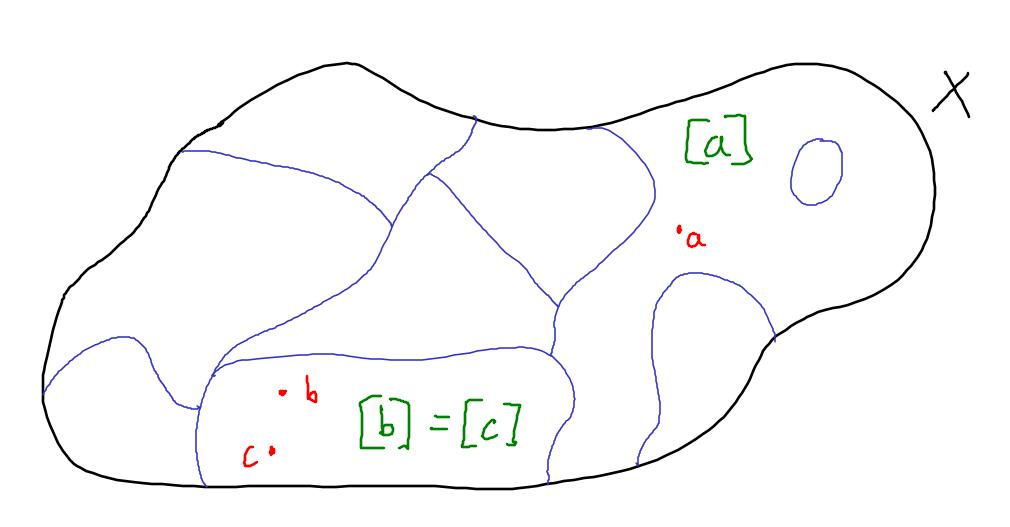
\includegraphics[width=12cm]{./_img/equivalence.jpeg}
	\caption{Die Menge $X$ zerfällt in disjunkte Äquivalenzklassen.}
\end{figure}


% --------------------------------------------------------------------
% §2 Section <<Aufgabenvorschlaege>>
% --------------------------------------------------------------------


\clearpage
\section{Aufgabenvorschläge}





\begin{aufg}[Konkrete Relationen]
Untersuche die folgenden Relationen darauf, ob sie reflexiv, symmetrisch, antisymmetrisch oder transitiv sind. Welche Relationen sind Äquivalenzrelationen, welche Halbordnungen, welche Totalordnungen? Sofern eine Äquivalenzrelation vorliegt, beschreibe die Äquivalenzklassen.
\begin{enumerate}[a)]
\item Es bezeichne $S$ die Menge aller Städte auf der Erde. Betrachte darauf die Relation
\begin{align*}
 A \sim B \quad& :\Leftrightarrow\quad \text{$A$ und $B$ sind höchstens 100km voneinander entfernt} && A,B\in S
\end{align*}
\item Auf der Menge $\Rz$ die Ungleichheitsrelation „$\neq$“.
\item Auf der Menge $\Rz$ die übliche „$<$“-Relation.
\item Es sei $M$ die Menge aller Menschen. Betrachte darauf die Relation
\begin{align*}
 a \sim b \quad& :\Leftrightarrow\quad \text{$a$ und $b$ haben (bzw. hatten) ein gemeinsames Kind} && a,b\in M
\end{align*}
\item Auf der Menge $\Zz$ die Teilbarkeitsrelation
\begin{align*}
 m\mid n \quad& :\Leftrightarrow\quad \exists c\in \Zz:\  c\cdot m=n && m,n \in \Zz
\end{align*}
\end{enumerate}
\end{aufg}


 
 
 
 
 \begin{aufg}[Abstrakte Relationen] \label{abstraktrel}
Untersuche die folgenden Relationen darauf, ob sie reflexiv, symmetrisch, antisymmetrisch oder transitiv sind. Welche Relationen sind Äquivalenzrelationen, welche Halbordnungen, welche Totalordnungen? Sofern eine Äquivalenzrelation vorliegt, beschreibe die Äquivalenzklassen.
\begin{enumerate}[a)]
	\item Auf einer beliebigen Menge $X$ die Gleichheitsrelation „$=$“.
	\item Für zwei Mengen $X,Y$ und eine beliebige Abbildung $f:X\to Y$ die Relation
	\begin{align*}
	 a\sim b \quad &:\Leftrightarrow\quad f(a)=f(b) && a,b\in X
	\end{align*}
          \item Auf einer beliebigen Menge $X$ die „Allrelation“, bezüglich der für alle $x,y\in X$ gilt, dass $x\sim y$. Verkörpert wird diese Relation durch die Teilmenge $X\times X\subseteq X\times X$.
        \item Auf einer beliebigen Menge $X$ die „leere Relation“, bezüglich der gar keine Elemente von $X$ zueinander in Beziehung stehen und die durch die Teilmenge $\emptyset\subseteq X\times X$ verkörpert wird.
\end{enumerate}
 \end{aufg}

 


\begin{aufg}[Graphen]
Bestimme, ob die Relationen, die durch die folgenden Graphen repräsentiert werden, reflexiv, symmetrisch, antisymmetrisch und/oder transitiv sind. Liegt sogar eine Äquivalenzrelation oder eine Ordnungsrelation vor?
\begin{figure}[H]
	\begin{tikzpicture}
		\begin{scope}[xshift=-6cm]
			\node (P0) at (-1,1) {$a$};
			\node (P1) at (-1,-1) {$b$};
			\node (P2) at (1,-1) {$c$};
			\node (P3) at (1,1) {$d$};
			\path[commutative diagrams/.cd, every arrow, every label]
			(P3) edge[commutative diagrams/loop] (P3)
			(P2) edge (P0)
			(P0) edge (P3)
			(P1) edge[<->] (P2);
		\end{scope}
		\begin{scope}[xshift=-2cm]
			\node (P0) at (-1,1) {$a$};
			\node (P1) at (-1,-1) {$b$};
			\node (P2) at (1,-1) {$c$};
			\node (P3) at (1,1) {$d$};
			\path[commutative diagrams/.cd, every arrow, every label]
			(P0) edge (P2)
			(P1) edge (P2)
			(P0) edge[<->] (P1);
		\end{scope}
		\begin{scope}[xshift=2cm]
			\node (P0) at (-1,1) {$a$};
			\node (P1) at (-1,-1) {$b$};
			\node (P2) at (1,-1) {$c$};
			\node (P3) at (1,1) {$d$};
			\path[commutative diagrams/.cd, every arrow, every label]
			(P1) edge[commutative diagrams/loop] (P1)
			(P2) edge[commutative diagrams/loop] (P2)
			(P3) edge[commutative diagrams/loop] (P3)
			(P0) edge[commutative diagrams/loop] (P0)
			(P1) edge[<->] (P2);
		\end{scope}
		\begin{scope}[xshift=6cm]
			\node (P0) at (-1,1) {$a$};
			\node (P1) at (-1,-1) {$b$};
			\node (P2) at (1,-1) {$c$};
			\node (P3) at (1,1) {$d$};
			\path[commutative diagrams/.cd, every arrow, every label]
			(P0) edge (P1)
			(P0) edge (P2)
			(P0) edge (P3)
			(P1) edge (P2)
			(P3) edge (P2);
		\end{scope}
	\end{tikzpicture}
\end{figure}
 \end{aufg}
 




\begin{aufg}[Äquivalenzklassen]
 Betrachte die beiden Abbildungen
 \begin{align*}
   f : \Rz^2 \to \Rz \ &,\ (x,y) \mapsto x+y \\
   g : \Rz^2 \to \Rz \ &,\ (x,y) \mapsto x^2+y^2
 \end{align*}
 Nach \cref{abstraktrel}b) sind durch
 	\begin{align*}
	 p\sim_f q \quad &:\Leftrightarrow\quad f(p)=f(q) && p,q\in \Rz^2 \\
	 p\sim_g q \quad &:\Leftrightarrow\quad g(p)=g(q) && p,q\in \Rz^2
	\end{align*}
zwei Äquivalenzrelationen $\sim_f$, $\sim_g$ auf $\Rz^2$ gegeben. Visualisiere die Äquivalenzklassen jeweils durch eine Zeichnung.
\end{aufg}



 \begin{aufg}[Laptops] \label{laptopaufg}
Zeige, dass auf der Menge $X$ aller Laptops die Relation \glqq\_ ist das gleiche Modell wie \_ \grqq eine Äquivalenzrelation ist. Verdeutliche Dir anhand des Beispiels noch einmal den Unterschied zwischen $X$ und $\sfrac{X}{\sim}$.
\end{aufg}

 
 \begin{comment}
\begin{aufg}[Parallelität]
Eine \textit{Gerade} $g$ in der Ebene $\Rz^2$ ist eine Menge der Form
\[ g= \left\{ x+ty \mid t\in\Rz \right\} \,, \]
wobei $x\in\Rz^2$ ein \textit{Ortsvektor} und $y\in\Rz^2$ ein \textit{Richtungsvektor} der Geraden genannt werden.

Auf der Menge aller Geraden in der Ebene $\Rz^2$ betrachten wir die Relation $g\parallel h :\Leftrightarrow$ $g$ ist parallel zu $h$, oder genauer: ein möglicher Richtungsvektor von $g$ ist ein Vielfaches eines möglichen Richtungsvektors von $h$. Ist etwa
\begin{align*}
	g&=\left\{x+ty\mid t\in\Rz \right\} & y&=\left\{u+tv\mid t\in\Rz\right\}
\end{align*}
für gewisse Vektoren $x,y,u,v\in\Rz^2$, so kannst Du annehmen
\[ g\parallel h \Leftrightarrow \exists r\in\Rz: y=rv \,. \]

Zeige, dass Parallelität auf der Menge aller Geraden in $\Rz^2$ eine Äquivalenzrelation bildet. Was sind die Äquivalenzklassen?
\end{aufg}
\end{comment}


%%% Local Variables:
%%% mode: latex
%%% TeX-master: "Skript"
%%% End:
